\newpage
\subsubsection{PCB Design}

The complete schematic and PCB layout are provided in 
Appendix~\ref{app:schematic}.

\paragraph{Layer Stackup}

The four-layer stackup consists of a top signal layer, a dedicated ground plane, a power plane, and a bottom signal layer.
The ground plane is kept continuous and unbroken across the full board area to give a uniform reference potential and minimise loop inductance.
Ground stitching vias are placed when signals transition between the top and bottom signal layers, ensuring the return current path remains close to the signal trace.
Signal traces are \qty{0.3}{\milli\meter} wide, while power traces carrying \qty{\pm 12}{\volt} from the Eurorack supply are widened to \qty{0.8}{\milli\meter} to handle the higher currents.

The top layer carries through-hole components forming the user interface and I/O: jacks, slide potentiometers, buttons, and WS2812 RGB LEDs.
SMD components are placed on the bottom layer, keeping the assembly compact and the top layer unobstructed.

\paragraph{Power Distribution}

The Eurorack \qty{\pm 12}{\volt} supply rails are decoupled at the board entry point with \qty{47}{\micro\farad} bulk capacitors to suppress low-frequency noise from the Eurorack power bus.
Each power pin of the codec and MCU is individually bypassed with a \qty{100}{\nano\farad} ceramic capacitor placed as close as possible to the pin to suppress high-frequency noise.

The \qty{3.3}{\volt} digital supply is generated by a buck converter followed by an LDO regulator.
The buck converter reduces the input voltage efficiently before the LDO. 
This minimizes power dissipation in the linear stage and reduces thermal load.
A separate, filtered analog supply rail \(3.3V_A\) is derived from the \qty{3.3}{\volt} rail using an Eaton MFBW1V series ferrite bead (\qty{120}{\ohm} at \qty{100}{\mega\hertz}) in series with a decoupling capacitor to ground.
This forms a low-pass filter that attenuates high-frequency switching noise from the digital supply before it reaches the codec analog domain.

The WS2812 RGB LEDs require a dedicated \qty{5}{\volt} supply, provided directly by the buck converter output.
A 74AHCT1G14DBVRG4 Schmitt trigger inverter is used to level-shift the \qty{3.3}{\volt} MCU data signal to the \qty{5}{\volt} logic level required by the WS2812 data input.
The \qty{5}{\volt} domain is distributed through a separate copper fill in the power plane, at the top portion of the board where the LEDs are located.

A LM4040DIM3X-10 shunt voltage reference provides a stable \qty{-10}{\volt} reference used for biasing the CV input summing amplifiers, as described in the CV input stage design (Section \ref{ref:cv-input-stage-design}).

\paragraph{Signal Integrity Considerations}

The board is divided into two functional regions: the analog frontend occupies the bottom portion of the PCB near the input and output jacks, while the digital domain, including the MCU and supporting circuitry, is placed in the top portion.
The codec is positioned between the two regions. 
This minimizes both the analog signal path length to the frontend and the I2S and SPI trace lengths to the MCU.

The buck converter is placed in the top portion of the board, as far as possible from the sensitive analog frontend.
The ground plane is cut out beneath the buck converter inductor to prevent switching noise from coupling into the ground plane through parasitic capacitance.

A \qty{1.27}{\milli\meter} pitch SWD header is placed on the back of the board, for programming and debugging via a standard ST-Link interface.

\paragraph{Design Errors and Revisions}

Two hardware errors were identified during bring-up of the first PCB revision.

The first concerns the gate input stage.
One GPIO pin assigned to a gate input was found to be unavailable on the STM32H7 \ac{EXTI} interrupt lines simultaneous to the other GPIO EXTI interrupts, making edge detection impossible in firmware for that channel.
To make the pin work with interrupts, the original pin is set up as floating in the firmware. A bodge wire connects the gate signal to an alternative GPIO that has EXTI capability.
This will be corrected in the next PCB revision by assigning the correct pin during schematic entry.

\begin{figure}[H]
    \centering
    \includegraphics[width=0.5\textwidth]{../images/hardware_design/bodges/gpio_wire_bodge.JPG}
    \caption{Bodge wire connecting the Gate 03 signal from PC9 to PC6 directly on the MCU pins.}
    \label{fig:gpio-bodge}
\end{figure}

The second error concerns the slide potentiometer LED indicators.
The KiCad component symbol for the slide potentiometers was created incorrectly based on a misreading of the datasheet pin assignment.
As a result, the LED anode is routed to a no-connect pin rather than the correct pad, leaving the LED indicators non-functional in this revision.
The potentiometer position readout is unaffected and functions correctly.
Both errors are documented and scheduled for correction in the next revision.

\begin{figure}[H]
	\centering
	\begin{minipage}{0.48\textwidth}
		\centering
		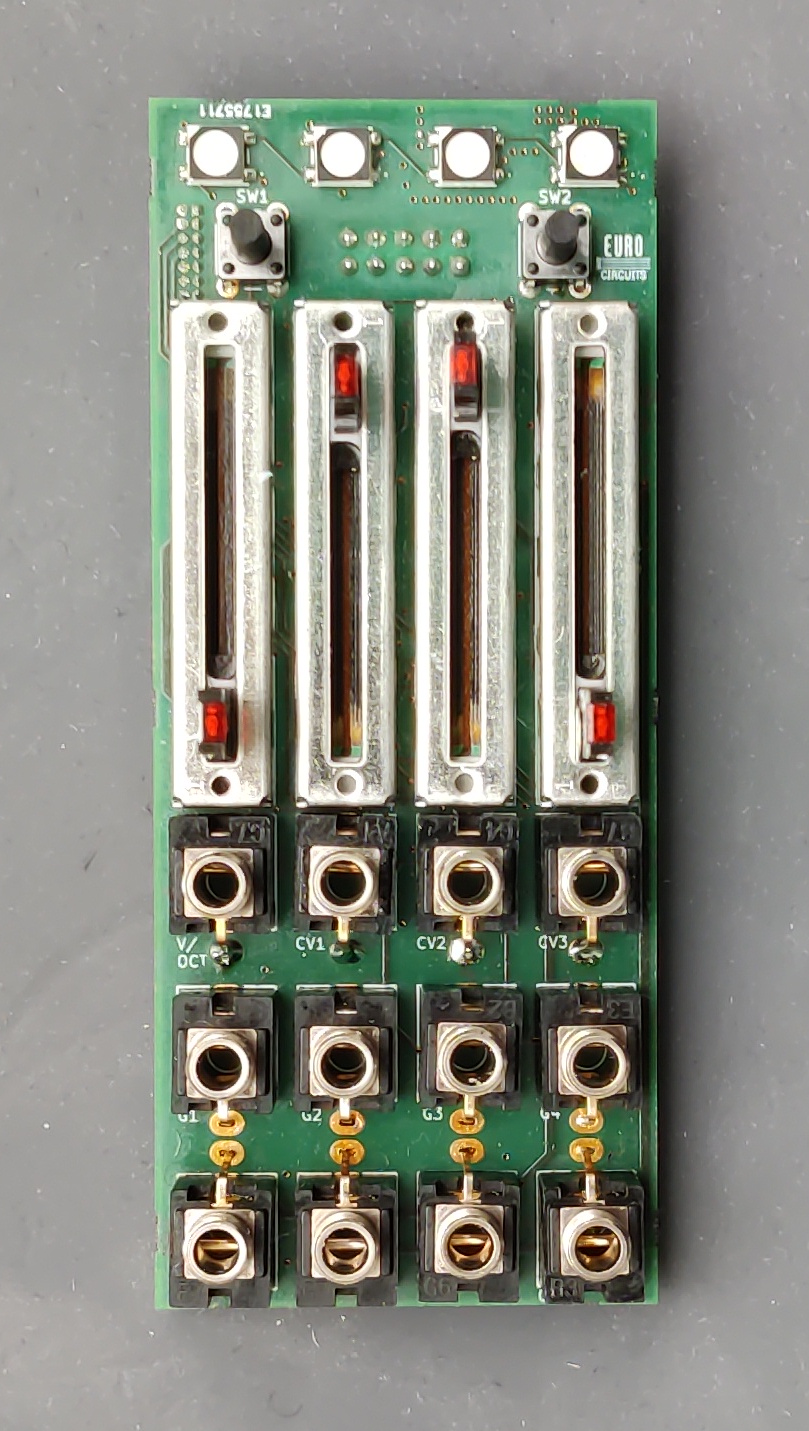
\includegraphics[width=0.7\textwidth]{../images/hardware_design/pcb_design/pcb_top.jpg}
		\subcaption{Top (mostly THT)}
	\end{minipage}
	\hfill
	\begin{minipage}{0.48\textwidth}
		\centering
		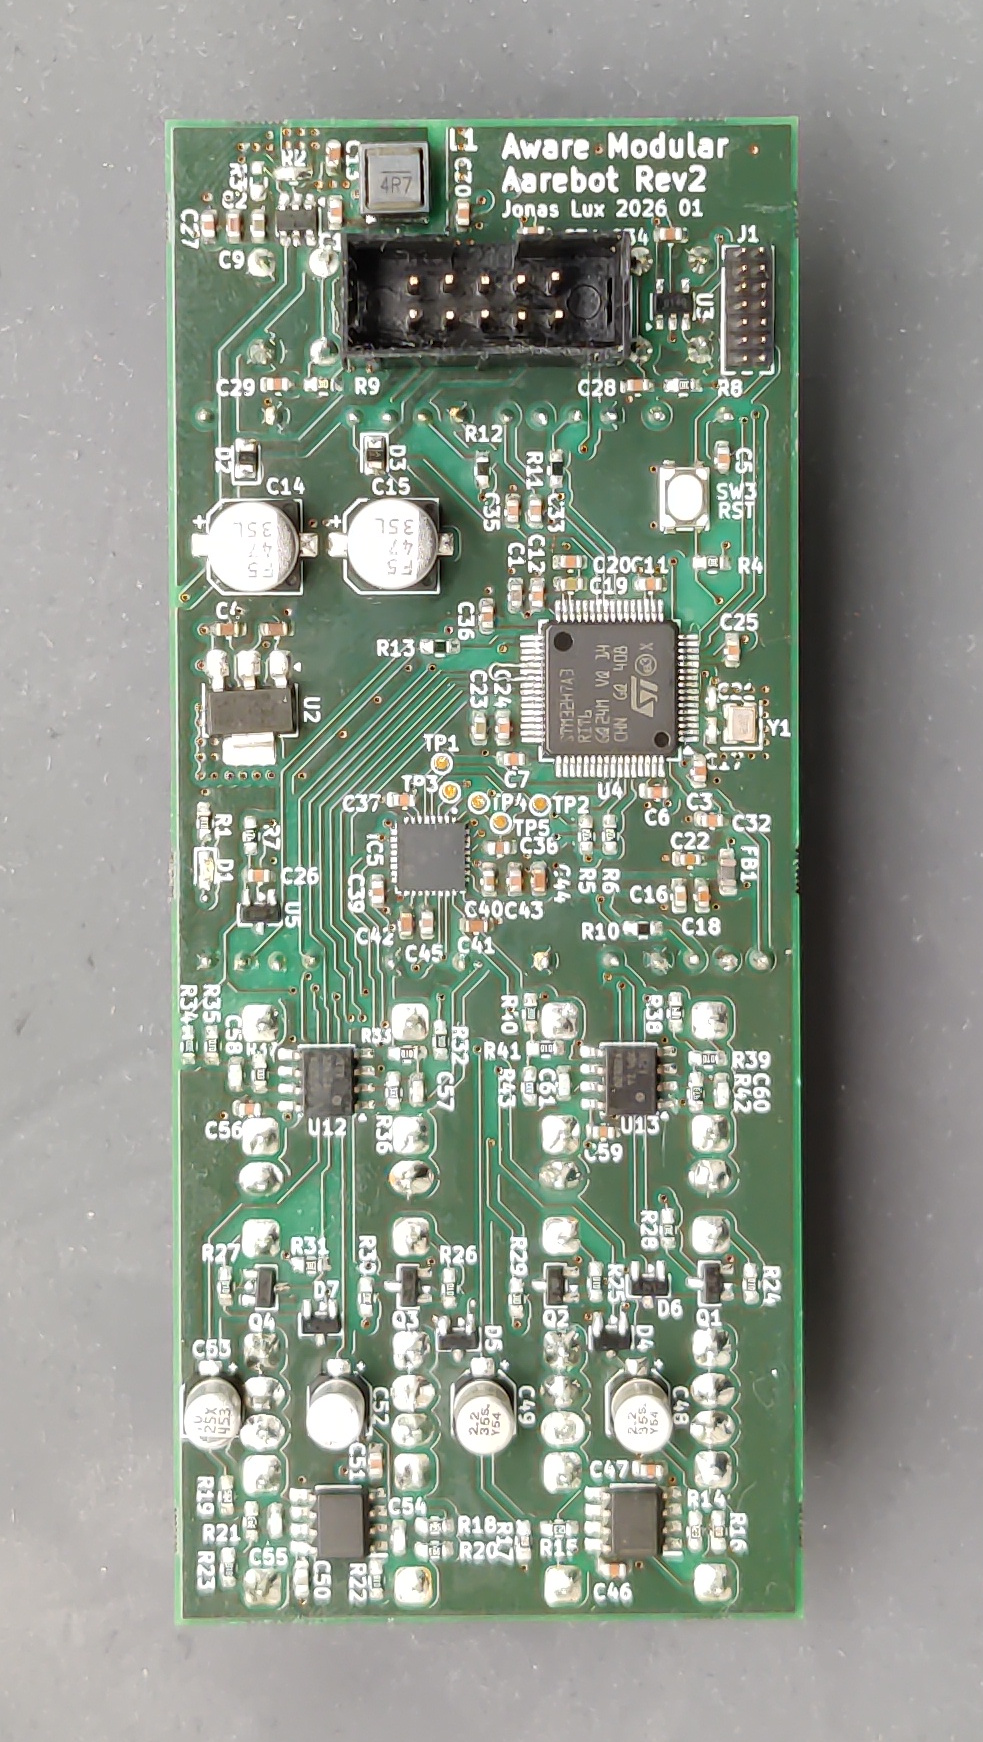
\includegraphics[width=0.7\textwidth]{../images/hardware_design/pcb_design/pcb_bot.jpg}
		\subcaption{Bottom (mostly SMD)}
	\end{minipage}
	\caption{Top and Bottom of soldered PCB -- all components in place}
	\label{fig:pcb_soldered}
\end{figure}

% TODO images of assembled PCB!
